%          spconf.sty  - ICASSP/ICIP LaTeX style file, and
%          IEEEbib.bst - IEEE bibliography style file.
% --------------------------------------------------------------------------
\documentclass{article}
\usepackage{spconf,amsmath,graphicx}
\usepackage{booktabs}
% Title.
% ------
\title{Applied machine learning system ELEC0132 20/21 report}
\name{SN: 17031141}
\address{}
%
\begin{document}
%
\maketitle
%
\begin{abstract}
    This section provides a brief overview of the methodology/results presented in the report.\footnote{The code is provided link-to-download-your-project.com and GitHub project: link-to-your-github-project}
\end{abstract}
%

%

\section{Introduction}
\label{sec:intro}
    Computer Vision is a very popular field of Machine Learning Systems and this report addresses 4 problems that was solved using both computer vision and machine learning techniques. This report will discuss the methodology that was adopted on the ``CelebA" dataset and the ``Cartoon Set" dataset for the following tasks:
    \begin{itemize}
    	\item Gender Classification
    	\item Emotion Recognition
    	\item Shape Classification
    	\item Colour Classification
    \end{itemize}

    The proposed method for gender recognition is to generate an Active Shape Model (ASM) of the sample image to extract the specific landmark features. This method specifically uses the dlib package and its 68 landmarks to extract features from the face. We will then use this data to train a model to be used for predicting test data.\\
    
    The task for emotion recognition was greatly simplified to just classifying whether the person in the image is smiling or not. So similarly with the method for gender recognition, the same ASM was used to extract features from the face, these features would then be fed into a model for training purposes to be used for predicting test data.\\
    
    Now for the cartoon set, the task was to classify one of five face shapes and one of five eye colours from the cartoon image. For the former case, the images were preprocessed to only contain the edges and from that information, the model could classify a cartoon image for face shape with reasonable accuracy.\\
    
    For the latter, the images were preprocessed to crop out all but one of the eyes of the image to focus the appropriate information and were then fed into a model for training.
\section{Literature survey}
\label{sec:lite}
    This section should focus on an overview of potential approaches to solve the tasks. You can introduce some classical and state-of-the-art machine learning algorithms.


\section{Description of models}
\label{sec:models}
    Here the machine learning model choice will be explained and justified for each task. 
    
    \subsection{Support Vector Machines}
    To explain briefly, any dataset that needs to be categorized can be plot onto a feature space with N number of dimensions. Decision regions need to be decided upon in order to separate the feature space into distinct categories as much as possible such that a datum can be categorized based on where it ends up in the feature space. This can be seen in Fig. \ref{fig:example_svm}
    
    \begin{figure}[htb]
    	\centering
    	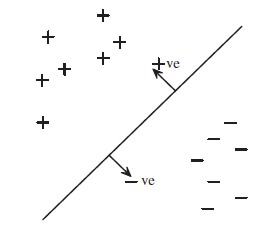
\includegraphics[scale=0.7]{Figures/Example_SVM.PNG}
    	\caption{Example of a decision region in a feature space from \cite{6812816} (Fig 1.1)}
    	\label{fig:example_svm}
    \end{figure}

    Now it can be seen in Fig. \ref{fig:example_svm} that the decision region can be moved slightly closer to either space and the classification would remain the same. The job of the SVM is the optimize this decision. Another thing to note here is that the decision boundary need not be a straight line (linear), it can fit other shapes as well. Namely polynomial lines of different degrees and a radial basis function. \\
    
    It can be quite intuitive here however, that using SVMs as a model should work well for discrete data that has clear and definitive categories i.e. a classification problem. Especially considering that for task A1, the problem is of binary classification, meaning that only two categories exist. From here we need to preprocess the data into the necessary details and size for an SVM model to analyse and categorise, the implementation of which will be shown in Section \ref{sec:impl}.
    
    \subsection{Convolutional Neural Networks}
    \begin{figure}[htb]
    	\centering
    	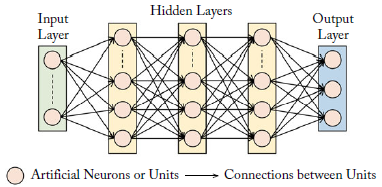
\includegraphics[scale=0.7]{Figures/Example_NN.PNG}
    	\caption{Example of fully connected feed forward neural network from \cite{8295029} (Fig 3.1)}
    	\label{fig:example_nn}
    \end{figure}
    
    It is shown in Fig.\ref{fig:example_nn} what an artificial neural network looks like. Data is fed into the input layer and then into each hidden layer. Each neuron in each layer performs a series of computations to transform the data and the modify by the neurons bias. Each neuron will have its own unique bias. At the output the predictions are compared with the true values using a cost function. The results of the cost function will be applied to all the layers to re-adjust the neuron biases and weights. In this way the model is trained.\\
    
    CNNs are just another type of neural network where some of the hidden layers will be convolutional layers. These layers perform the operation of convolution onto the data to extract features. The kernel size used for convolution can be specified such that CNNs are very useful when the data involves images. It can extract the necessary features in the learning process. The specific architecture used will be shown in Section \ref{sec:impl}.\\
    
    Here, the image preprocessing techniques are far less complex as the CNN can do much of it for you. This means that while training time could be longer, preprocessing time is much shorter than it would be. This is convenient because once the model has been trained, testing it on raw data should not take long. So in terms of practicality the CNN may be more fitting to use.\\
    
    \subsection{K-Means Clustering}
    \textbf{08227986}\\
    Traditionally, CNNs and SVMs are used for supervised learning. This means that the proper labels have been designated to each input datum beforehand and the model will learn based on this. Unsupervised learning is when the proper labels are not pre-designated. The model, therefore has to perform pattern recognition to see what kind of classification/categorisation can be performed on the training set.\\
    \begin{figure}[htb]
    	\centering
    	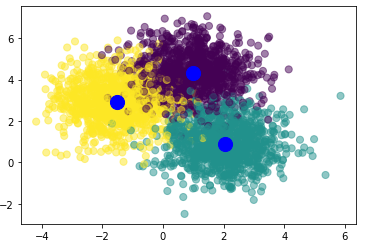
\includegraphics[scale=0.7]{Figures/Example_KMeans.PNG}
    	\caption{Example of K-Means Clustering from the sklearn package in Python}
    	\label{fig:example_kmeans}
    \end{figure} 

	Here in Fig. \ref{fig:example_kmeans} it can be seen that 3 clusters have been specified and have been used to categorise the data. The model will find the natural groupings among the data samples. Now this seems more intuitive to use for multi-class classification problems than SVMs as it will find the geometric distance of the datum from all of the cluster centres/means and classify it as the shortest one.\\
	
	 The issue with this however is that this model is intended for unsupervised learning and our problem is of a supervised learning nature. Despite this, it is still worth considering as a model because you can specify the initial cluster centres and the method to calculate the geometric distances.\\
	 
	  The idea behind this is that you can take 5 images from the cartoon set for which the labels are 0-4 respectively and use that data as the cluster centres. Upon learning with more and more data, the clusters will expand and the centres will change position but if learnt correctly the new centres should not vary in position too greatly from the initial setting.
	  
    \subsection{Task A1: Gender Detection}
    For this particular task, two models were implemented and tested. Firstly, an SVM model was tested because it is a binary classification problem. This would mean that only one decision boundary has to be generated so by far it should be the simplest model to generate. The preprocessing for this particular model involves using an Active Shape Model (ASM) generated by the dlib package. This particular ASM has only 68 landmarks but the performance is quite reasonable and can be seen in Section \ref{sec:results}. \\
    
    However, despite the fact that human beings can generally tell apart genders, the landmark information from any face will appear to overlap in some aspects due to both samples simply having a human face. This would mean that the decision boundary for the SVM would probably not be as simple as a linear function. \\
    
    The other model implemented was a CNN. The reasoning behind this is that the data samples we are looking at involve RGB images of resolution (178x218). There is quite a lot of literature explains that CNNs are quite advantageous when used on images for image classification \textbf{8295029}. 
    \subsection{Task A2: Emotion Recognition}
    This task has a lot of similarities with A1 in that it is from the same dataset and that it is a binary classification problem. So for the same reasons both an SVM model and a CNN model will be used. The difference being that the CNN architecture will be different as the feature desired from the image is different.
    \subsection{Task B1: Face Shape Recognition}
    This task is a multi-class classification problem. The dataset is also very simple in the sense that every image has the same format and structure. Due to these reasons. An SVM model and a K- Means Clustering model was used to solve this problem.\\
    
     Due to the many classes, the SVM model will be more complex than the previous two tasks but as the label designation is still discrete, an SVM model can work quite well with minimal preprocessing techniques due to the simplicity of the dataset.\\
    
     K-Means Clustering was also used because we have the ability to initialise the cluster centres before they are updated in the learning process. So the preprocessing involved would be simply finding 5 samples from the dataset with unique labelling. 
    \subsection{Task B2: Eye Colour Recognition}
    Here the task is similar in nature to B1 but quite different to the other 2 tasks because in this task, the colour dimension plays an essential role for classification. In the previous cases, colour was not required and therefore the images were converted to grayscale in order to reduce the size of the data load and speed up the preprocessing. \\
    
    Due to this, the models being used here are SVM and CNN. The classification is still discrete so SVM can still work and because the feature required from the images is very clear and simple to extract, a low complexity CNN architecture can be used.

\section{Implementation}
\label{sec:impl}
	\subsection{The Data}
	The two datasets used for these tasks were the CelebA dataset and the Cartoon Set.
	\subsubsection{CelebA}
	Each image in this set has the dimensions 178x218 pixels and depicts a human being with the focus being on their face. The faces have multiple different angles to the camera. They also vary in gender, race, hair length, accessory (glasses). 
	\subsubsection{Cartoon Set}
	Each image in this set has the dimensions 500x500 pixels and depicts a cartoon face looking directly head from the computer screen. The base structure for each image is essentially the same with a randomized face shape, skin colour, eye colour, facial hair and hair style along with seeing eye glasses and sun glasses. The original dataset has 10 classes for face shape and eye colour but these tasks will only be looking at 5 of these 10 classes in both categories.  
    \subsection{Common External Libraries Used}
    In this section I will detail the common external libraries used to generate and train my machine learning models.\\
    
    For the SVM models, the \verb|Scikit-Learn| library was used, also better known as \verb|sklearn|. This package came in quite handy as it already has a class \verb|svm| which can be imported. Additionally it contains the \verb|metrics| class which can be used to easily measure the accuracy score with the predefined functions.\\
    
    Although it could have been hard coded the \verb|train_test_split| function from \verb|sklearn| helped in splitting the dataset into the necessary proportions to be tested.\\
    
    Another important library that was used for the SVM models was \verb|pickle|. It is compatible with \verb|sklearn| models and was used to serialize the trained model and save it such that time would not be wasted having to train the model on every test.\\
    
    Now for the CNN models the libraries \verb|Keras| and \verb|Tensorflow| were essential. Each layer used in any of the CNN architectures can be found as objects in the \verb|Keras| package
    \subsubsection{SVM}
	Here some additional libraries were used:
	\begin{itemize}
		\item \verb|dlib|
		\item \verb|os|
		\item \verb|numpy|
		\item \verb|cv2|
		\item \verb|skimage|
	\end{itemize}
	The \verb|dlib| package was very useful in that it allows you to generate a shape predictor using an in built function and a .dat file with the essential facial landmarks written in.\\
	The \verb|numpy| package was very useful as the images are read in as matrices or arrays and the package enables a lot of matrix transformations and analysis of matrix properties.\\
	The \verb|cv2| and \verb|os| libraries were used to read in the images and convert it to grayscale as the colour dimension of the image is not necessary for the task.\\
	The \verb|skimage| library were useful for the functions it has to transform an image, particularly the \verb|hog| function
    \subsubsection{CNN}
    Some addition libraries used here were:
    \begin{itemize}
    	\item \verb|pandas|
    	\item \verb|matplotlib|
    \end{itemize}
    The \verb|pandas| library was very helpful in reading the labels file into a data-frame. A data-frame is quite convenient to use when manipulating and preprocessing the labels file.\\
    The \verb|matplotlib| library was useful in plotting the convergence when training the model. 
    \subsection{Task A1: Gender Detection}
	\subsubsection{SVM Training Pipeline}
	 First the labels are read into a dictionary using the file names (without extension) as the key and the gender label as the translation. Then using the filenames from the dictionary keys and the \verb|os| package, the images are read in from the correct directory one by one and fed into a function.\\
	 
	 The function will convert the image to grayscale using the \verb|cv2| package and then a \verb|dlib| computation is run on the grayscale image to draw rectangles on where the \verb|dlib| algorithm predicts a face to be. The landmarks are applied to image in the rectangles. The coordinates of the rectangle on the full image are extracted as well as the width and height. The function then returns the landmarks inside the rectangle with the largest area, the area calculated with the coordinates and dimensions of the rectangle from earlier.\\
	 
	 An entire matrix is generated composed of the features of every image in the dataset given. In parallel, a labels matrix is generated with the gender label for each image with the same length as the feature matrix and perfectly aligned indices. These matrices are then split using the \verb|train_test_split| method from the \verb|sklearn| package with a ration of 0.25 test data.\\
	 
	 A model classifier is generated using the \verb|sklearn| package with a \textit{polynomial} kernel of degree 3 and a hyper-parameter of 1. This classifier is then fit to the training data and labels. The accuracy of the model is seen when using the \verb|predict| method from the \verb|sklearn| package with the test data and test labels split from earlier.\\
	 
	 It should be noted that due to the size of the dataset and the resolution of the image, the preprocessing of this dataset takes quite long. It was also attempted to downscale the images to 45x55 before grayscaling them in order to reduce computational and time cost. The results for both can be found in Section \ref{sec:results} and Table \ref{table:Table1}.

 	\subsubsection{CNN Training Pipeline}
 	Firstly \verb|pandas| was used to read in the labels file into a data-frame. Then using some \verb|pandas| methods the binary labelling of gender was replaced with one hot encoding. This new data-frame with one-hot encoding was then randomised and split into training, validation and testing data-frames with 6:2:2 ratio using the \verb|numpy| package.\\
 	
 	Then each of these data-frames were used in the \\ \verb|ImageDataGenerator| class from \verb|keras| with the following parameters: target\_size=(55,45), batch\_size=30,\\ color\_mode=grayscale, interpolation=bicubic.\\
 	
 	This was done because the \verb|ImageDataGenerator| class is quite a convenient format for data to be fed into the CNN for training and testing. The CNN architecture used is shown in Table \ref{table:A1_Arch}. The learning rate was set to 0.0001 and the \textit{Adam} optimizer was used with a loss function of \textit{Binary Cross-entropy}.\\
 	
 	 The model is then fit using the training and validation generators. The model was initially trained for 25 epochs and the results would then be plotted on a graph using the \verb|matplotlib| package features to observe the convergence. The results of the training and testing can be found in Section \ref{sec:results}.
 	
 	\begin{table}[]
 		\begin{tabular}{|c|c c c|}
 			\hline
 			Input Layer & size = 55x45 	&				&	\\
 			\hline
 			Convolution & filters = 96 	& kernel = 4x4 	& actv = ReLU\\
 			\hline
 			Max Pool	&				& pool = 2x2  	& \\
 			\hline
 			Batch Norm. & 				&				&\\
 			\hline
 			Convolution & filters = 256 & kernel = 3x3 	& actv = ReLU\\
 			\hline
 			Max Pool	&				& pool = 2x2	&\\
 			\hline
 			Batch Norm. &				&				&\\
 			\hline
 			Convolution & filters = 256 & kernel = 2x2	& actv = ReLU\\
 			\hline
 			Flatten 	& 				& 				&\\
 			\hline
 			Dense 		& filters = 512 &				& actv = ReLU\\
 			\hline
 			Dropout 	&	rate = 0.2 	&	 			&\\
 			\hline
 			Dense 		& filters = 512 &				& actv = ReLU\\
 			\hline
 			Dropout 	& rate = 0.2 	& 				&\\
 			\hline
 			Output Layer& filters = 2 	&				& actv = SftMx\\
 			\hline
 		\end{tabular}
 	\caption{A1 CNN Architecture}
 	\label{table:A1_Arch}
 	\end{table} 
    \begin{figure}[htb]
		\centering
		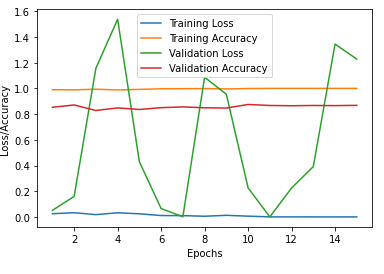
\includegraphics[scale=0.7]{Figures/A1_CNN_Graph.PNG}
		\caption{A1 CNN Learning Curve}
		\label{fig:A1_curve}
	\end{figure} 	
    \subsection{Task A2: Emotion Recognition}
    Seeing as the task for A2 is very similar to A1, the same training pipeline and image preprocessing techniques is utilised for the SVM model. This is because of the 68 landmarks, some of them are dedicated to the lips of the face of the subject. There fore the same feature extraction can be used.\\
    
    For the CNN model however, the feature being analysed is quite different to A1 so a different neural network architecture is used and it can be seen in Table \ref{table:A2_Arch}.
 	\begin{table}[]
	\begin{tabular}{|c|c c c|}
		\hline
		Input Layer & size = 55x45 	&				&	\\
		\hline
		Convolution & filters = 100 & kernel = 3x3 	& actv = ReLU\\
		\hline
		Batch Norm. & 				&				&\\
		\hline
		Max Pool	&				& pool = 2x2  	& \\
		\hline
		Convolution & filters = 200 & kernel = 2x2 	& actv = ReLU\\
		\hline
		Batch Norm. &				&				&\\
		\hline
		Max Pool	&				& pool = 2x2  	& \\
		\hline
		Convolution & filters = 400 & kernel = 2x2	& actv = ReLU\\
		\hline
		Flatten 	& 				& 				&\\
		\hline
		Dense 		&filters = 1024 &				& actv = ReLU\\
		\hline
		Dropout 	& rate = 0.2 	&	 			&\\
		\hline
		Dense 		& filters = 512 &				& actv = ReLU\\
		\hline
		Dropout 	& rate = 0.2 	& 				&\\
		\hline
		Output Layer& filters = 2 	&				&actv = SftMx\\
		\hline
	\end{tabular}
	\caption{A2 CNN Architecture}
	\label{table:A2_Arch}
	\end{table}
    \begin{figure}[htb]
    	\centering
    	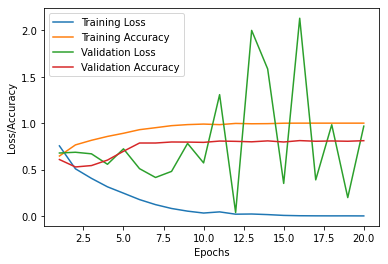
\includegraphics[scale=0.7]{Figures/A2_CNN_Graph.PNG}
    	\caption{A2 CNN Learning Curve}
    	\label{fig:A2_curve}
    \end{figure} 
    \subsection{Task B1: Face Shape Recognition}
    Task B1 is very similar to A1 and A2 in the sense that similar features need to be extracted from the images for training purposes. The differences are that this is now a multi-class classification problem and that the 68 landmarks used in tasks A1 and A2 are not as accurate for cartoon faces and therefore are not as effective for feature extraction as other methods.\\
    
    The method chosen here is to extract the \textit{Histogram of Oriented Gradients} (HOG) from each image and use this data to train the model. An example of the resulting HOG image can be seen in Figure \ref{fig:hog}.
    \begin{figure}[htb]
    	\centering
    	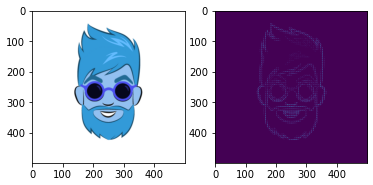
\includegraphics[scale=0.7]{Figures/Hog_Example.PNG}
    	\caption{Example of HOG image from Cartoon Set}
    	\label{fig:hog}
    \end{figure} 
    
    \subsubsection{SVM Training Pipeline}
    Similarly to the CNN implementations from earlier tasks, pandas is used to read in the labels file into a data-frame. All rows after the 1000th are dropped from the data-frame in order to save on preprocessing and training time as 10000 images that are all 500x500 pixels in size is a very large data size to process. A data-frame is used here instead of a dictionary like in the previous cases because it was found to be easier to debug the importing of the data and the indexing of the labels and images.\\
    
    The data-frame is then randomised and split into training : validation : test with the ratios 6 : 2 : 2. The new data-frames were then used to import the appropriate images to the labelling in the data-frames. The \verb|hog| operation was performed on each images and stored into a feature matrix that would then be used to train, validate and test the model. In parallel to the \verb|hog| operation, a label matrix was being generated as well with the same indices as the feature matrix.\\
    
    The training features and training labels are then used to train the model. The model has been set as an SVM model with a \textit{polynomial} kernel of degree 3 and with the hyper-parameter set to 1. The validation and test feature matrices and labels are used to validate and test the model performance. The results can be seen in Table \ref{table:Table1}.
    \subsection{Task B2: Eye Colour Recognition}
    Task B2 differs quite vastly from tasks A1 and A2 because, the dataset is of cartoon images, the problem is of multi-class classification and finally that colour plays an important role in this problem. If the dataset was of real humans then some correlation would be found with skin tone, facial structure, hair colour and eye colour. \\
    
    However this is not the case here, seeing as the image features are randomised for the cartoon, the eye colour itself must be directly analysed. This can be seen in Figure \ref{fig:eye}.
    \begin{figure}[htb]
	\centering
	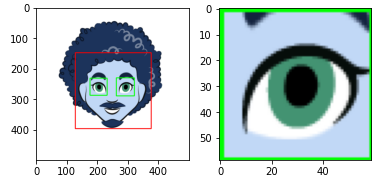
\includegraphics[scale=0.7]{Figures/Eye.PNG}
	\caption{Example of extracted eye from full image}
	\label{fig:eye}
\end{figure}     
	This technique is accomplished through the use of \textit{Haar Cascades} from the \verb|cv2| library. A face cascade is used over the image to detect a face. Once that has been found, a rectangle is drawn around the face and the future operations reside within this rectangle. An eye cascade is performed inside the rectangle to detect eyes and if found, a rectangle is drawn around that.\\
	
	Then using the coordinates of both rectangles, everything from the image except the eye is cropped, leaving us with the region of interest.  
	\subsubsection{SVM Training Pipeline}
	Similar to task B1 in the SVM case, the labels are preprocessed the same way and the images are imported the same way. The difference now is that each image is cropped to only contain the right eye. The cropped image is then converted from BGR colour space to HSI colour space because using the image on its own is too many dimensions for the SVM to train on.\\
	
	The average hue of each eye is then added to a feature matrix. The feature matrix and the label matrix is then used to train the SVM. It is found experimentally that an SVM with a \textit{Radial Basis Function} (RBF) kernel and hyper-parameters set to 50 produces the best performance as seen in Figure \ref{fig:B2_SVM}.
	\begin{figure}[htb]
		\centering
		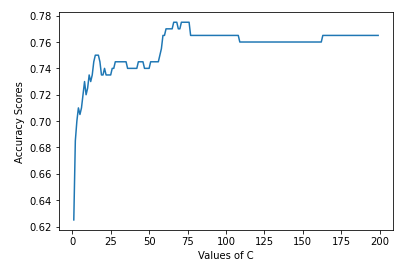
\includegraphics[scale=0.7]{Figures/B2_SVM_C.PNG}
		\caption{Graph of Accuracy against Hyper-Parameter for an RBF kernel}
		\label{fig:B2_SVM}
	\end{figure}
	\subsubsection{CNN Training Pipeline}
	The labels are imported in using \verb|pandas| into a data-frame. This data-frame is then modified such that the eye colour is classed using one hot encoding rather than from 0-4. This data-frame is then split into train, validate and test with the 6:2:2 ratio and used to import the images and preprocess them as stated above.\\
	
	The difference to the SVM case for B1 is that the cropped region of interest is not converted to HSI colour space as the average hue is not needed in this case. The cropped region of interest and the accompanying labels are simply fed into the CNN using the \verb|ImageDataGenerator| class. The CNN architecture can be seen in Table \ref{table:B2_Arch}.
 	\begin{table}[]
	\begin{tabular}{|c|c c c|}
		\hline
		Input Layer & size = 56x56 	&				&	\\
		\hline
		Convolution & filters = 100 & kernel = 2x2 	& actv = ReLU\\
		\hline
		Max Pool	&				& pool = 2x2  	& \\
		\hline
		Batch Norm. & 				&				&\\
		\hline
		Flatten 	& 				& 				&\\
		\hline
		Dense 		&filters = 512 &				& actv = ReLU\\
		\hline
		Dropout 	& rate = 0.2 	&	 			&\\
		\hline
		Dense 		& filters = 512 &				& actv = ReLU\\
		\hline
		Dropout 	& rate = 0.2 	& 				&\\
		\hline
		Output Layer& filters = 2 	&				&actv = SftMx\\
		\hline
	\end{tabular}
	\caption{B2 CNN Architecture}
	\label{table:B2_Arch}
\end{table}
\begin{figure}[htb]
	\centering
	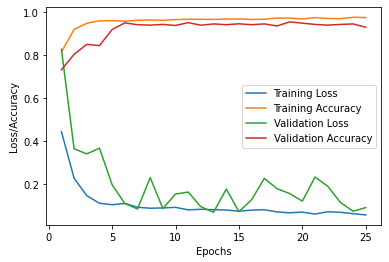
\includegraphics[scale=0.7]{Figures/B2_CNN_Graph.PNG}
	\caption{B2 CNN Learning Curve}
	\label{fig:B2_curve}
\end{figure}	
\section{Experimental Results and Analysis}
\label{sec:results}
    The results of each model case for the tasks can be found in Table \ref{table:results}. It can be observed that in most cases the training accuracy is best with a CNN model but the testing accuracy is best with an SVM model.\\
    
     For tasks A1 and A2 it takes approximately 3 hours to generate the feature matrix of the full 5000 images from the dataset. This will be because the functions used to generate the coordinates of the 68 landmarks are quite complex in time (from observation at least $O(n^3)$ timing complexity). Right now the functions use a brute force tactic to generate the landmarks but if a more efficient algorithm was used then this will save a lot of time.\\
     
     Another point to be made is that it is unlikely for task A2 that the model will need the full 68 landmarks to detect whether the subject is smiling or not accurately. This can be observed in Figure \ref{fig:landmarks}. Theoretically you should only need the landmarks centred around the jaw and the lips. The rest of the landmarks are useless and need not be calculated, with this some time should be saved in generating the feature matrix for A2.\\
     \begin{figure}[htb]
     	\centering
     	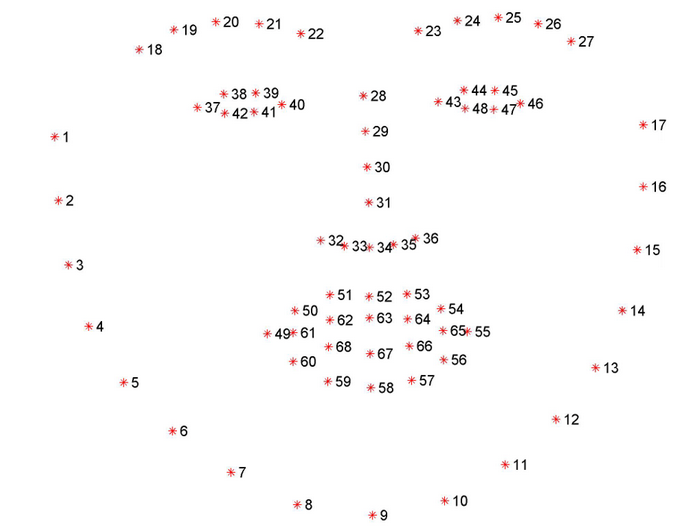
\includegraphics[scale=0.4]{Figures/landmarks.PNG}
     	\caption{Visual representation of the 68 landmarks from dlib}
     	\label{fig:landmarks}
     \end{figure}
 
  	The preprocessing for the other tasks runs fairly quickly because little preprocessing is required and that which is there is not very computationally intensive. It does take longer to train the CNN models over the SVM models but here one could trade-off complexity of the network for performance of the model. 
    \begin{table}[]
    \begin{tabular}{@{}lllll@{}}
    \toprule
    Task & Model & Train Acc & Val Acc & Test Acc \\ \midrule
    A1   & SVM   & 92.92\%   & 91.24\% & 92.67\%         \\
    A1   & CNN   & 99.73\%   & 85.70\% & 85.50\%         \\
    A2   & SVM   & 88.92\%   & 86.47\% & 89.68\%         \\
    A2   & CNN   & 100.0\%   & 80.10\% & 79.00\%         \\
    B1   & SVM   & 100.0\%	 & 98.60\% & 99.12\%		 \\
    B2   & SVM	 & 77.50\%	 & 75.82\% & 74.00\%		 \\
    B2   & CNN	 & 97.50\%	 & 92.98\% & 97.90\%		 \\ \bottomrule
    \end{tabular}
	\caption{The accuracy of each model for each task}
	\label{table:results}
    \end{table}

\section{Conclusion}
\label{sec:conc}
    In this work, six functioning machine learning models have been built and trained using the CelebA dataset and the Cartoon Set for four unique tasks. Tasks A1 and A2 involved gender detection and emotion detection on the CelebA dataset and the best model for both of these tasks seems to have been an SVM model with a polynomial kernel and hyper-parameter of 1. The image preprocessing done for both of these tasks is identical but the techniques used causes a great bottleneck in the training and testing of the model.\\
    
    Tasks B1 and B2 involved face shape recognition and eye colour recognition respectively, on the Cartoon Set. It was found that the SVM model with an RBF kernel and hyper-parameter of 75 was the best option for task B1. The best option for task B2 was a CNN with the architecture shown in Table \ref{table:B2_Arch}. The preprocessing done on the Cartoon Set for B1 was simply to apply the HOG operation onto each image. The preprocessing done on the same dataset for B2 was to isolate the eye using Haar Cascades and to use only the eye as the input to the CNN.

% References should be produced using the bibtex program from suitable
% BiBTeX files (here: strings, refs, manuals). The IEEEbib.bst bibliography
% style file from IEEE produces unsorted bibliography list.
% -------------------------------------------------------------------------
\bibliographystyle{IEEEbib}
\bibliography{ref}

\end{document}
